\documentclass[12pt]{article}

\usepackage{graphicx}
\usepackage{cgw04}
\usepackage{fancyhdr}

\title{Out-of-core problems}
\author{Tomasz Duszka, Jakub Janczak \small{ \em{ [duszka,janczak]@student.uci.agh.edu.pl} } }
\date{1 May 2005}

\pagestyle{fancy}

\rhead{http://www.ds14.agh.edu.pl/$\sim$kubek2k/ooc/}
\lhead{}

\begin{document}
\maketitle

\smallskip
\begin{figure}[h!]
	\begin{center}
		\includegraphics[scale=1.0]{tea.eps}
	\end{center}
	\smallskip
\end{figure}

\begin{center}
\begin{quotation}
	\noindent \em{,,The only way to discover the limits of the possible is to go
	    beyond them into the impossible.''}\cite{2ndclarkelaw}

	\hfill \textbf{--- Arthur C. Clarke \footnote{English physicist \& science fiction author (1917 - )}} \\
\end{quotation}
\end{center}
\begin{abstract}
%tu bedzie abstract
	In this paper we show out-of-core problems and some issues connected with it.
	As the OOC is a very wide matter, we are concerning on only some problems. 
	The main part of the paper are examples which are very useful in exploring OOC world. 
	There is also a chapter about OOC problem's solving environments.


\end{abstract}

\section{Introduction to Out-of-core problems}

\chapter{Wst�p}

SOA (Service Oriented Architecture) to najwi�ksze osi�gni�cie informatycznej my�li architektonicznej ostatnich lat\footnote{ ``My thought was, this change has to be compared to the switch from Newtonian physics to relativistic physics.''\cite{soa:newton}}.
Ten wprowadzony w 1996 roku przez Gartnera\cite{soa:gartner} paradygmat stanowi obecnie dominuj�cy nurt w projektowaniu system�w informatycznych\footnote{Ocenia si�, �e w ci�gu najbli�szych dw�ch lat znajomo�� technologii wspieraj�cych tworzenie aplikacji o architekturze SOA podwoi si� z 25 do 50\%\cite{soa:soa_adoption_eweek}} 
i jest ukoronowaniem wysi�k�w maj�cych na celu uproszczenie oprogramowania rozproszonego. Jego powstanie ma �cis�y zwi�zek z dynamiczn� ewolucj� architektur oprogramowania (por. rysunek \ref{fig:soa-ewolucja}).

\begin{figure}[htp!]
 \centering
 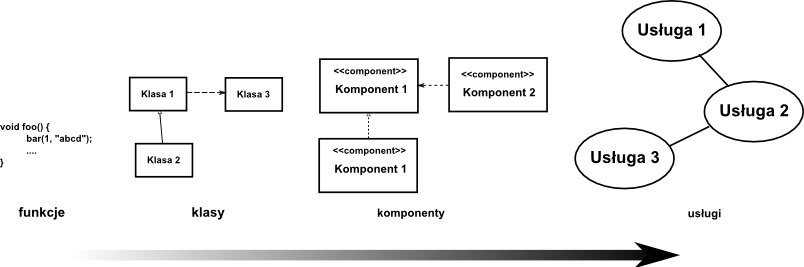
\includegraphics[bb=0 0 386 128]{intro/arch-evo.png}
 \caption{Ewolucja architektur oprogramowania \cite{soa:ibm_soma}}
 \label{fig:soa-ewolucja}
 % arch-evo.png: 427x142 pixel, 94dpi, 11.55x3.84 cm, bb=0 0 327 109
\end{figure}

Rosn�ce wymagania odno�nie mo�liwo�ci, jak i prostoty obs�ugi aplikacji, nieuchronnie prowadz� do wzrostu ich z�o�ono�ci.
Aktualny model tworzenia oprogramowania powoli osi�ga kres swoich mo�liwo�ci
- obserwowany jest znaczny wzrost koszt�w zwi�zanych z rozwi�zywaniem problem�w czysto technologicznych, np. integracj� system�w zbudowanych w oparciu o r�ne platformy po�rednicz�ce (z ang. middleware). In�ynierowie musz� r�wnie� radzi� sobie z ci�g�ymi naciskami organizacyjnymi i biznesowymi takimi jak: ograniczanie koszt�w wytwarzanego oprogramowania, potrzeba szybkiej odpowiedzi na zmieniaj�ce si� wymagania, mo�liwo�� �atwej integracji i absorpcji nowych partner�w biznesowych.
W celu zniwelowania wymienionych trudno�ci powsta�o szereg rozwi�za�, np. architektury przeznaczone do tworzenia system�w rozproszonych, przeno�ne j�zyki programowania, �rodowiska wspieraj�ce integracj� system�w itp.
Nie rozwi�zuj� one jednak wsp�czesnych problem�w - na przeszkodzie staje du�a r�norodno�� platform programistycznych, stosowanych technologii oraz rosn�ca potrzeba integracji system�w.
Brak uniwersalnego i powszechnie stosowanego, a jednocze�nie odpowiadaj�cego obecnym potrzebom rozwi�zania cz�stkowego, przyczyni� si� do powstania koncepcji SOA
- architektury zorientowanej na us�ugi (Service Oriented Architecture). Podstawow� zasad� rz�dz�c� tym podej�ciem jest lu�ne powi�zanie (z ang. loose coupling) pomi�dzy elementami systemu, pozwalaj�ce na proste komponowanie go jako ca�o�ci (zmian� w sposobie projektowania oprogramowania obrazuje \nolinebreak{rysunek \ref{fig:soa-evo2}}).

\begin{figure}[htp]
 \centering
 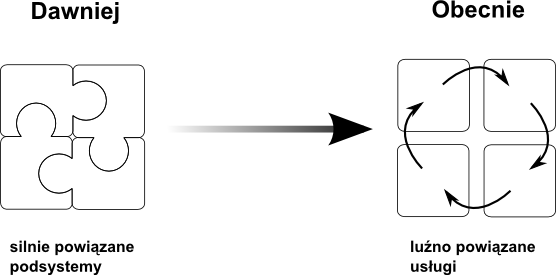
\includegraphics[bb=0 0 267 132]{intro/soa-evolution.png}
 \label{fig:soa-evo2}
 \caption{Zmiana w podej�ciu do projektowaniu oprogramowania}
 % soa-evolution.png: 348x172 pixel, 94dpi, 9.42x4.65 cm, bb=0 0 267 132
\end{figure}

Logiczn� konsekwencj� takiego podej�cia jest zastosowanie szeregu dobrych konwencji in�ynierskich, takich jak ukrycie implementacji\footnote{zwane te� autonomiczno�ci�} czy ponowne u�ycie (z ang. software reuse), przy jednoczesnym wzro�cie elastyczno�ci,  przejrzysto�ci, �atwo�ci wprowadzania zmian oraz prostocie zarz�dzania.

Powszechne uznanie SOA, spowodowa�o zmian� w kierunku rozwoju technologii z zakresu wymiany danych i integracji oprogramowania.
Coraz wi�kszy udzia� w rynku maj� te rozwi�zania, kt�re wi�ksz� uwag� przywi�zuj� do wsp�dzia�ania r�nych platform i przeno�no�ci. Chc�c realizowa� ide� SOA, u�yte technologie musz� dawa� jak najwi�ksz� swobod� w zakresie komunikacji. Ich baz� przestaje by� interfejs programistyczny konkretnego j�zyka, \nolinebreak{a zaczyna} format wymienianych danych. Dodatkowo chc�c zapewni� jak najwi�ksz� niezale�no�� poszczeg�lnych cz�ci system�w, coraz wi�kszy nacisk k�adzie si� na ukrywanie szczeg��w implementacji.

Od czasu opublikowania paradygmatu SOA w 1996 roku, powsta� szereg koncepcji (np. technologia webservice) maj�cych na celu praktyczn� realizacj� SOA.
W oparciu o nie, korzystaj�c jednocze�nie z idei ESB (Enterprise Service Bus) oraz j�zyka BPEL (Business Process Execution Language), firmy informatyczne s� w stanie stworzy� oprogramowanie spe�niaj�ce za�o�enia tej architektury,
obni�aj�ce jednocze�nie koszty rozwoju i utrzymania, jakie nale�a�oby ponie�� przy zastosowaniu tradycyjnego podej�cia.

Budowa oprogramowania w oparciu o technologie realizuj�ce SOA, wi��e si� z narzutami natury wydajno�ciowej. 
% , kt�re mog� by� nieakceptowalne w jego p�niejszym wykorzystaniu.
Jednocze�nie, brak powszechnej wiedzy na temat SOA i utartych dobrych wzorc�w wytwarzania powoduje, �e cz�sto oprogramowanie tworzone w tej architekturze, nie jest napisane w spos�b optymalny, bez wykorzystania jej podstawowych zalet.
Powa�nym wyzwaniem staje si� zatem kwestia pomiaru wydajno�ci tworzonych aplikacji\footnote{Brak zrozumienia kryteri�w wydajno�ciowych jest uznawany za jedno z pi�ciu najwi�kszych zagro�e� SOA \cite{soa:piec_zagrozen}}.

Do tej pory �wiat informatyczny nie dopracowa� si� jednolitej metodologii pomiar�w wydajno�ci system�w o architekturze SOA. Z punktu widzenia in�ynier�w oprogramowania - niemo�liwe jest obecnie przeprowadzenie analizy por�wnawczej takiego oprogramowania.
Istniej�ce rozwi�zania pozwalaj� na pomiary wydajno�ci poszczeg�lnych element�w systemu o architekturze SOA\footnote{Na rynku istnieje szczeg�lnie du�o rozwi�za� do testowania wydajno�ci oprogramowania opartego na technologii webservice}, jednak�e tematyka kompleksowego rozwi�zania tego problemu, nie spotka�a si� dotychczas z du�ym zainteresowaniem, zar�wno ze strony �wiata komercyjnego, jak i naukowego.

\section{Cel pracy}
Celem pracy jest analiza problemu pomiaru wydajno�ci aplikacji zbudowanych w oparciu o paradygmat SOA. Rozwa�onych zostanie kilka potencjalnych rozwi�za� oraz przeanalizowane zostan� zalety i wady ka�dego z nich.
W oparciu o postawiony w pracy zestaw wymaga� zostanie wybrane i zaimplementowane najlepsze.
 % a najlepsze rozwi�zanie zostanie wybrane w oparciu o postawiony w pracy zestaw wymaga�.
Stworzona implementacja zostanie sprawdzona w �rodowisku testowym na zestawie przyk�adowych aplikacji. Proces testowania i wyniki b�d� podstaw� do wyci�gni�cia wniosk�w na temat przydatno�ci wybranego rozwi�zania w analizie wydajno�ci aplikacji opartych o SOA.

\section{Struktura pracy}
Niniejsza praca rozpoczyna si� opisem technologii wykorzystywanych w tworzeniu aplikacji opartych o SOA. W rozdziale 3 szczeg�owo sformu�owano problem oraz zbi�r wymaga� stawianych poszukiwanemu rozwi�zaniu. 
Rozdzia� zawiera ponadto dyskusj� potencjalnych rozwi�za� wraz z ich wadami i zaletami. Wybrane jest jedno, kt�re najlepiej spe�nia postawione wymagania. W rozdziale 4 omawiane s� szczeg�y technologiczne implementacji wybranego rozwi�zania, natomiast w rozdziale 5 wyniki analizy przyk�adowej aplikacji w �rodowisku testowym. Prac� ko�czy rozdzia� 6 zawieraj�cy zbi�r konkluzji odno�nie mo�liwo�ci zastosowania i dalszego rozwoju zaimplementowanego systemu do badania wydajno�ci aplikacji o architekturze SOA.

Rozdzia�y 2.1, 2.2, 3.1, 4, 5.1, 5.5 oraz dodatek A zosta�y napisane przez Tomasza Duszk�. Rozdzia�y 1, 2.3, 2.4, 3.2, 3.3, 3.4, 5.1, 5.2 zosta�y napisane przez Jakuba Janczaka. Pozosta�e rozdzia�y: 6, 7 oraz 8 zosta�y napisane przez autor�w pracy wsp�lnie.
 
%  Rosn�ce nak�ady najwi�kszych gospodarek i �wiatowych koncern�w na systemy komputerowe sprawi�y �e
%  przekroczy�y one swoje naturalne granice. Rozwijaj�cym si� koncernom przesta�o wystarcza� wewn�trzne
%  wspomaganie ich dzia�ania - coraz wi�kszy udzia� w rynku maj� aplikacje zwyczajowo zwane B2B (Business
%  to Business) - maj�ce na celu wymian� informacji pomi�dzy r�nymi podmiotami. Poza tym przemys�, wraz
%  ze wzrostem zaawansowania, rozmiaru i udzia�u oprogramowania zaczyna si� boryka� z problemami jakich
%  wcze�niej nie do�wiadcza�:
% 
% 
% \begin{itemize}
% \item  szybko rozwijaj�cy si� rynek stymuluje powstawanie wielu coraz lepszych i pewniejszych technologii, co w istocie jest pozytywne, ale powoduje i� oprogramowanie ju� napisane bardzo szybko traci na warto�ci i aktualno�ci. Co poza wzrostem wydatk�w mo�e nawet, przy �le prowadzonej polityce doboru, spowodowa� konieczno�� wymiany ca�ych system�w
% \item  silnie zintegrowane systemy wymagaj� ci�g�ej konserwacji, a zmiany w jednej cz�ci zazwyczaj propaguj� si� na pozosta�e 
% \item  coraz wi�ksze skomplikowanie system�w powoduje, i� coraz trudniej je zrozumie� i rozwija�
% \end{itemize}
% 
% \subparagraph{Kr�tki wst�p do SOA}
% 
% SOA (Service Oriented Architecture) to koncepcja kt�rej za�o�enia uwalniaj� oprogramowanie od tych problem�w. SOA promuje model programowania zwany "lu�nym powi�zaniem", tj. komponenty opgramowania s� niezale�nymi bytami (us�ugami), kt�re komunikuj� si� mi�dzy sob� z pomoc� dobrze zdefiniowanych interfesj�w. Us�ugi te wymieniaj� mi�dzy sob� informacje samoistnie lub kierowane przez zewn�trzny proces koordynuj�cy. Praktyka pokaza�a, �e wdro�enie SOA w systemach wielkiej skali przynios�o wiele wymiernych korzy�ci takich jak
% % \footnote{za http://blogs.sun.com/rtenhove/entry/why_soa i http://labs.jboss.com/file-access/default/members/jbossesb/freezone/resources/whitepapers/WhyESB.pdf}:
% 
% \begin{itemize}
% \item  wielokrotne u�ycie komponent�w systemu 
% \item  szybkie reakcje na zmieniaj�ce si� wymagania i realia rynkowe - zmiana w procedurach biznesowych najcz�ciej powoduje zmian� w sposobie wywo�ywania us�ug, a nie ich wewn�trznej implementacji
% \item  mo�liwo�� stosowania przyrostowych metodologii rozwoju oprogramowania - w ostatnim czasie najpopularniejszych w firmach IT, dzi�ki kt�rym mo�liwe jest testowanie cz�sciowej, ju� wykonanej implementacji systemu
% \item  redukcja nak�ad�w poniesionych na oprogramowanie (o czym wspomnieli�my wcze�niej)
% \item  skupienie si� na innowacjach zamiast na konserwacji systemu 
% \end{itemize}
%  Podstaw� powstania SOA jest fakt i� na topie przestaje by� silna integracja, a zaczyna kompozycja :

% img /home/kubek2k/public{\textunderscore}html/dokuwiki/data/media/magisterka/wstep/ewolucja{\textunderscore}soa.png
% 
% 
% 
% \dokutitleleveltree{Problemy z SOA i pr�by rozwi�zania}
% \label{b9e3a44b7fdd9fd1d66bc1fc86f6286e}%% problemy_z_soa_i_proby_rozwiazania
%  Pomimo swoich licznych zalet, podej�cie SOA niesie ze sob� r�wnie� du�a ilo�� problem�w. Chc�c zapewni� wsp�dzia�anie system�w korzystaj�cych z r�nych technologii jeste�my skazani na stosowanie oprogramowania ��cz�cego (z ang. \hyperref[b200f0642a4dc4d9d66162920860c3f0]{middleware}) kt�re jest w je nam w stanie zapewni� - poci�ga to jednak za sob� do�� du�e narzuty czasowe. Zwyczajowo technologi� u�ywan� do integracji system�w w architekurze SOA stosuje si� technologi� \hyperref[742523daef59db4b718409f46de05d0c]{WebService'�w} opartych o protok� \hyperref[cbf4e0b7971051760907c327e975f4e5]{SOAP}. Dodatkowo wykorzystanie samej architektury SOA nak�ada na tworz�cych konieczno�� zaszywania lokalizacji poszczeg�lnych komponent�w systemu (tj. ka�da z us�ug musi wiedzie� gdzie powinna skierowa� kolejne ��dania, w zale�no�ci od otrzymanych danych).
% 
% 
% \dokutitlelevelfour{BPEL}
% Chc�c zmieni� naturalne podej�cie do wykonywania ci�gu operacji na rozproszonych us�ugach (tzw. choreografii), wprowadzono poj�cie orchiestracji. \hyperref[54f21b6ecfc3292b6bcc669edc745133]{Orchiestracja} polega na tym, �e z komponent�w systemu spada konieczno�ci bycia �wiadomym o otoczeniu - wprowadzone zostaje poj�cie procesu biznesowego kt�ry sam wie co ma robi� z danymi, i zawiaduje sekwencjami wywo�a�. Zmian� podej�cia mo�na por�wna� do przej�cia z modelu \hyperref[705bcf0e77bc8b6fc8e66cbf3c055e6c]{peer-to-peer} do modelu scentralizowanego.
% 
% Jednym z rozwi�za� wspieraj�cych ide� orchiestracji jest j�zyk BPEL - Business Process Execution Language. Dzi�ki niemu jeste�my w stanie modelowa� nawet bardzo z�o�one procesy biznesowe na r�nych stopniach abstrakcji, korzystaj�c ze standardowych element�w sk�adniowych znanych z innych j�zyk�w programowania. Co najwa�niejsze zosta� on pomy�lany w taki spos�b, aby modele da�o si� przedstawi� w postaci graficznej - bloczk�w, dzi�ki czemu proces tworzenia aplikacji ulega bardzo znacznemu uproszczeniu, a zarazem powi�ksza si� grono potencjalnych u�ytkownik�w. Nie bez znaczenia jest r�wnie� obecno�� du�ej gamy narz�dzi do modelowania w BPEL.
% 
% Co wa�ne standard ten jest bardzo silnie wspierany przez przemys� informatycznym i bez w�tpienia b�dzie w najbli�szym czasie b�dzie to jedyny sensowny wyb�r na tym polu. Liczby \dokufootnote{ankieta OASIS: \href{http://mult.ifario.us/p/bpel-adoption-thermometer}{http://mult.ifario.us/p/bpel-adoption-thermometer}} pokazuj�, i� w�r�d programist�w tworz�cych systemy SOA 23\% korzysta, a 28 planuje u�ywa� BPEL w swoich aplikacjach \dokufootnote{z drugiej strony 40\% nadal nie wie co to BPEL, co pokazuje nam jak niedojrza�y jest jeszcze ten rynek}. Liczby te rosn� z roku na rok. \dokufootnote{wi�cej informacji o BPEL \hyperref[22ee86570f52c823bdb1d5ef39aed4f7]{tutaj}}
% 
% 
% \dokutitlelevelfour{ESB}
% Innym, wspomnianym wcze�niej, problemem jest mnogo�� u�ywanych technologii w zewn�trznych i ju� istniej�cych systemach (tzw. systemach odziedziczonych). Cz�sto okazuje si�, �e pomimo najwi�kszych stara� nie jest mo�liwe dostosowanie si� do takowych, a architektura SOA oparta tylko i wy��cznie na \hyperref[742523daef59db4b718409f46de05d0c]{Web Service'ach} zaczyna traci� na swoich w�asno�ciach. Rozwi�zania mog� by� dwa:
% 
% 
% \begin{itemize}
% \dokuitem  prostsze - mo�na stworzy� opgramowanie opakowuj�ce (tzw. wrapper) dla danej us�ugi, zrzucaj�c na siebie tym samym konieczno�� zmian za ka�dym razem kiedy ta us�uga zmieni si�
% \end{itemize}
% lub
% 
% 
% \begin{itemize}
% \dokuitem  bardziej z�o�one, ale daj�ce wi�kszy zysk w przysz�o�ci - mo�na u�y� istniej�cych platform integracyjnych (tzw. "integration middleware")
% \end{itemize}
% \hyperref[efb03b68f7a0c2a331fc61a491c4b2d7]{ESB (Enterprise Service Bus)} jest w�a�nie jedn� z takich platform. Jej idea opiera si� na istnieniu szyny danych przy pomocy kt�rej realizujemy wszystkie komunikacje w systemie. Dzi�ki temu to nie proces, a szyna mo�e decydowa� o tym gdzie ma trafi� dana informacja. Takie dzia�anie daje bardzo du�e mo�liwo�ci, szczeg�lnie je�li chodzi o przeno�no�� poniewa� chc�c skorzysta� z jakiej� us�ugi proces nie odwo�uje si� do konkretnej instancji, ale po prostu wysy�a odpowiednio spreparowan� wiadomo�� do szyny i oczekuje na odpowied�. Dzi�ki takiem podej�ciu znacznie prostsze staje si� zapewnienie wielu wa�nych w�a�ciwo�ci systemu rozproszonego:
% 
% 
% \begin{itemize}
% \dokuitem  integracja z innymi technologiami - ujednolicenie "punktu styku" ze �rodowiskiem zewn�trznym i istniej�cymi systemami, za pomoc� odpowiednich adapter�w i konwerter�w wiadomo�ci
% \dokuitem  rozwi�zanie problemu lokalizacji us�ug - to szyna decyduje gdzie wys�a� dan� wiadomo��  zatem nasze aplikacje staj� si� przeno�ne, wszystko zale�y od konfiguracji ESB
% \dokuitem  dzi�ki zastosowaniu redundantnych us�ug i odpowiedniej konfiguracji jeste�my wstanie zapewni� wy�sz� wydajno�� i niezawodno�� systemu
% \dokuitem  dzieki temu, �e dane pod��aj� niejako jednym kana�em komunikacyjnym �atwiejsze staje si� zarz�dzanie bezpiecze�stwem 
% \end{itemize}
%  Mimo swojej kr�tkiej historii koncepcja ESB udowodni�a ju� swoj� przydatno�� w budowaniu du�ych system�w. ESB jest z powodzeniem wdra�ane w wielu inicjatywach ze szczeg�lnym uwzgl�dnieniem du�ych projekt�w rz�dowych \dokufootnote{np. \href{http://www.gcn.com/print/25_20/41319-1.html}{system dla policji stanu Washington} czy \href{http://newsroom.progress.com/phoenix.zhtml?c=86919&p=NewsArticle&id=997931}{systemy bukmacherskie w UK}} \dokufootnote{wi�cej informacji o ESB \hyperref[efb03b68f7a0c2a331fc61a491c4b2d7]{tutaj}}
% 
% 
% \dokutitleleveltree{Podsumowanie}
% \label{96e21bf66c0133beafda0ff9f011643e}%% podsumowanie
% Jak wida� rynek informatyczny poradzi� sobie z g��wnymi problemami z kt�rymi spotyka si� programista stosuj�cy architektur� SOA. Jednak otaczaj�c ju� w samym sobie "ci�k�" technologi� \hyperref[742523daef59db4b718409f46de05d0c]{WebService'�w} dodatkowymi rozwi�zaniami, ryzykujemy sytuacj� w kt�rej to ich narzut b�dzie mia� bardzo znacz�cy udzia� w wykonaniu tych operacji. Dodatkowo zagro�eniem dla tych technologii jest (sic!) ich dynamiczny rozw�j w ostatnich latach\dokufootnote{co tyczy si� w zasadzie ca�ego rynku oprogramowania na �wiecie} - istnieje zagro�enie, �e producenci oprogramowania popychani coraz wi�ksz� konkurencj� na rynku, k�ad� wi�kszy nacisk na mo�liwo�ci pomijaj�c tak istotne cechy jak odporno�� na b��dy czy wydajno��. 
% 
% Chc�c por�wna� dzia�anie r�nych rozwi�za�, tudzie� sprawdzi� narzut wynikaj�cy z wdro�enia danej technologii, musi istnie� jaka� sp�jna metodologia pomiar�w wydajno�ci - kt�rej rynek do tej pory niedopracowa� si�. 
% 
% Celem tej pracy jest pokazanie jakie podej�cie nale�y zastosowa� do pomiar�w wydajno�ci system�w o architekturze SOA. Efektem pracy ma by� r�wnie� stworzenie narz�dzia do takich pomiar�w, oraz opracowanie przyk�adowych wynik�w test�w w oparciu o przyk�adow� aplikacj� stworzon� w oparciu o wymienione wcze�niej technologie.
% 
% 
% \dokutitleleveltwo{Koniec}
% \label{44943fe207611d5625258c1059d25ec8}%% koniec
% Napisa� o mo�liwym narzucie generowanym przy takiej ilo�ci technologii i konieczno�ci pomiar�w.
% 
%  Chc�c omin�� problemy z integracj� system�w stworzonych z u�yciem r�nych technologii i operuj�cych w r�nego rodzaju �rodowiskach, jako standard w zastosowaniach architektury SOA przyj�o si� stosowa� technologi� \hyperref[cca5d72b2013a1b8737449a4dd328903]{WebSevice'�w}. U�ycie tak "ci�kiego" podej�cia do zdalnego korzystania z us�ug ma jednak bardzo du�e prze�o�enie na wydajno�� aplikacji. Z tego powodu istotnie wa�nym staje si� fakt i� brak jest zunifikowanego podej�cia do badania jak wydajne s� aplikacje spe�niaj�ce za�o�enia SOA. Taki stan rzeczy dodatkowo daje argument tzw. SOA-sceptykom, kt�rzy jako g��wn� wad� tej architektury wymieniaj� w�a�nie straty wydajno�ciowe. 
% 
% Celem tej pracy b�dzie opracowanie takiego podej�cia ze szczeg�lnym uwzgl�dnieniem aplikacji opracowanych w oparciu o BPEL\ldots{}. i nie wiem co tu dalej napisac ;)
% 
% "My thought was, this change has to be compared to the switsch from Newtonian physics to relativistic physics." - \href{http://weblogs.asp.net/ralfw/archive/2005/07/03/417507.aspx}{http://weblogs.asp.net/ralfw/archive/2005/07/03/417507.aspx}
% 
% Melted Cheese programming - przej�cie z SOA - \href{http://msdn2.microsoft.com/en-us/library/ms954609.aspx}{http://msdn2.microsoft.com/en-us/library/ms954609.aspx}
% 
% [mniej patetycznie, wi�cej konkret�w, gar�� fakt�w]
% 
%  Dodatkowym problem, kt�ry jest szczeg�lnie istotny w obecnych czasach, to du�a pr�dko�� rozwoju przemys�u i technologii informatycznych. Cz�sto okazuje si� �e technologia traci swoj� warto�ci na przestrzeni miesi�cy.  


\section{Problems and solving examples}


\subsection{Out of core sorting}

Sorting is a fundamental procedure, useful in many various tasks.
It's very important to be able to efficiently sort large datasets using limited memory size.

One of possibilities to implement out-of-core sort may be the external merge sort.
This algorithm is a recursive procedure as follows.
In each recursion we check if current list fits entirely in physical memory.
If so, we read entire list into main memory, sort it and write it back to disk in contiguous place.
If not, we split current list into k sublists of equal sizes, sort each one recursively and then merge all sublists into one sorted list.
Of course, main problem of this algorithm is the merging process, which must be done in an IO efficient way.
We keep k buffers (each one for each sublist), which are initially initialised with first blocks of each sublist.
Then we perform merging of items in k buffers (each buffer is already sorted) and output sorted items to disk.
When some buffer is exhausted it is loaded with the next buffer from the corresponding sublist.
This process continues until all of the k sublists are merged.

Let's denote input list size as n and size of one IO buffer as b.
As we can see complexity of this algorithm is $O(n\log{n})$.
The IO complexity is $\displaystyle O(\frac{n}{b}\log_{k}\frac{n}{b})$.
By choosing right k we can minimalise IO communication.


\subsection{OOC LU and QR factorization}


As described in \cite{ooc-scalapack} out-of-core extension of ScaLAPACK exists which provides three core factorization routines: LU, QR and Cholesky.
They allow factorization of dense systems which are too large to fit in psychical memory. 
Original matrix is stored entirely on disk and factorization routines transfer its parts into memory. 
These routines make use of portable I/O interface and ScaLAPACK in-core factorization as a subroutines.

Authors of \cite{ooc-scalapack} also provide comparison between various problems size for out-of-core factorizatoin routines. 
They used Linux cluster, each node consisted of dual Pentium II at 450MHz with 512MB and a local 8GB IDE disk using red-hat Linux 6.2 with smp kernel.

Below there is a comparison for LU factorization applied to various matrices and grids.
The 'fact' time is the total elapsed to perform out-of-core factorization, 
the 'solve' is the total elapsed time for solution with 10 vectors (they both include I/O time) and
the 'io' is the total elapsed time for read and write operations.
\bigskip

\begin{center}
\begin{tabular}{|r|r|r|r|r|} \hline
    size & grid & fact & solve & io \\ \hline
    
    16000 & 4 x 4 & 3670s & 180s & 417s \\
    32000 & 4 x 4 & 28850s & 508s & 1918s \\ \hline
    
    16000 & 4 x 8 & 1867s & 123s & 163s \\
    32000 & 4 x 8 & 15730s & 313s & 951s \\
    40000 & 4 x 8 & 32420s & 443s & 1595s \\ \hline
    
    20000 & 8 x 7 & 2301s & 81s & 78s \\
    32000 & 8 x 7 & 8317s & 289s & 470s \\
    45000 & 8 x 7 & 22508s & 482s & 1148s \\
    80000 & 8 x 7 & 128155s & 899s & 3627s \\ \hline    
    
    
\end{tabular}
\end{center}
\bigskip

As shown in the table, the time for the I/O operations was generally a small fraction of overall time. 
This shows that these out-of-core algorithms were compute-bound on this cluster. 


\subsection{Compression and decompression of large n-dimensional scalar fields}


Many scientific applications make use of extremely large data sets, usually 
represented as n-dimensional scalar fields. For example, a typical 3D simulation
may require regular grid of $2048^{3}$ samples. Such grids need to be
stored and transmitted ie. to remote visualisation clients, which may take
large amount of time due to their big sizes. In such case variety of data compression
techniques may be used to reduce data size.

Of course several compression techniques exists for lower dimensional gridded data,
like JPEG and others. Many method for 4D volumes were also proposed in recent years ie.
wavelets, Discrete Cosine Transform or Run Length Encoding.

Recent research showed that there exists another algorithm, suitable for arbitrary
n-dimensional scalar fields \cite{ndim-fields}. It's based on the Lorenzo predictor.
It estimates the scalar value of a sample on the corner of an n-dimensional cube
from the scalar values of the others $2^{n}-1$ corners. The value of the scalar field
F(u) is estimated using the following formula:
\bigskip

$E(v)=\displaystyle \sum_{u \in U} (-1)^{c_{0}(u)+1}F(u)$
\bigskip

The estimated value computed from this formula in n-dimension is exact
for all scalar functions that are polynomial of degree n-1.

Compressor in each step estimates next value in the scanline order and encodes the difference
between the original and estimated value (which usually requires less bits). These differences
may be encoded ie. with an adaptative arithmetic encoder.

As proved in \cite{ndim-fields} this algorithm may be easily adapted to out-of-core problems.
In fact, if properly written it requires only about $D^{n-1}$ bytes of memory for compressing (or decompressing)
scalar field of $D^{n}$ bytes size. For example, if we want to compress scalar field of $2048^3$ values
(each encoded in one byte which gives us 8GB size) we need only about 4MB memory window for this algorithm, and
resulting compression is generally comparable to wavelet compression.

\subsection{Inverting great matrices}

Matrix inversion is used in many applications ie. as a direct method for solving linear equations.
For challenging applications (like astronomical simulation, crash test simulation, global climate modelling and many others) the memory is always insufficient in size.
Scientist usually want to increase accuracy which causes bigger and bigger matrices.
Thus, out-of-core algorithm for inverting matrices might be very useful.

Inversion of a matrix can be computed from its LU factorization.
LU factorization produces matrices: L (lower triangular) and U (upper triangular) such that:
\bigskip

$M = LU$
\bigskip

In general when LU decomposition uses partial pivoting there may be third matrix P, which stores the permutation matrix.

We're searching for a matrix $M^{-1}$ such that:
\bigskip

$MM^{-1}=I$

$LUM^{-1}=I$
\newline

$LY=I$

$UM^{-1}=Y$
\bigskip

Firstly we compute matrix Y such that $LY=I$, this can be done using backward substitution.
Another backward substitution is used to compute $M^{-1}$ from $UM^{-1}=Y$

As proved in \cite{matinv} out-of-core inverting of a matrix can be efficiently done using blocked decomposition of matrices.
It presents algorithms for both parallel out-of-core LU factorization (which is also presented in \cite{ooc-scalapack}) and parallel out-of-core triangular substitution.
\bigskip

\begin{center}
\begin{tabular}{|r|r|r|r|r|r|r|} \hline
    size & grid & LU fact & io & communication & computation & total \\ \hline
    
    12288 & 1x8 & 29m39s & 10m16s & 11m19s & 21m21s & 1h36m \\ \hline
	& 2x4 & 21m17s & 9m39s & 4m31s & 20m27s & 1h12m \\ \cline{2-7}
	& 4x2 & 18m50s & 8m52s & 4m30s & 19m50s & 1h08m \\ \cline{2-7}
	& 8x1 & 19m57s & 8m09s & 9m17s & 19m50s & 1h21m \\ \hline
    20480 & 1x8 & 2h37m & 1h07m & 1h27m & 2h34m & 10h38m\\ \hline
	& 2x4 & 1h06m & 1h02m & 31m55s & 2h05m & 6h23m \\ \cline{2-7}
	& 4x2 & 1h50m & 1h02m & 17m48s & 1h56m & 6h21m \\ \cline{2-7}
	& 8x1 & 1h43m & 55m46s & 27m26s & 1h49m & 6h25m \\ \hline
    27648 & 1x8 & 7h59m & 2h07m & 6h16m & 4h04m & 1d04h \\ \hline
	& 2x4 & 4h34m & 1h59m & 2h10m & 3h51m & 16h45m \\ \cline{2-7}
	& 4x2 & 3h20m & 2h02m & 49m31s & 3h47m & 12h43m \\ \cline{2-7}
	& 8x1 & 3h02m & 2h04m & 53m28s & 3h46m & 12h29m \\ \hline
    
\end{tabular}
\end{center}
\bigskip

These results were obtained on a cluster of 8 PC-Celeron running Linux (each one has 96MB of psychical memory) and interconnected by a Ethernet switch,
Of course there is a way to avoid I/O overhead in this algorithm, it can be done by overlapping I/O with the computation, which is further described in \cite{matinv}
\bigskip

\subsection{Processing big meshes}

Polygonal meshes acquired with modern scanning technology can easily reach hundreds of millions of triangles which gives many GB data size.
There exist special approaches to processing such large meshes, which sizes often exceeds 4GB address space of 32-bit machines.
Those approaches may be divided into few groups \cite{mesh}:
\bigskip

\begin{itemize}

    \item{mesh cutting} - original mesh is cut into smaller parts, small enough to fit entirely in memory.
	Then algorithm analyses each part independently.
	Despite the simplicity of this approach, the initial cutting step can be expensive when the input mesh is given in an indexed representation. 
	Unfortunately mesh cutting typically lowers the quality of the output and there might be some problems with processing cut boundaries.
	
    \item{batch processing} - stream the data through main memory in one or more passes.
	Of course computations are restricted to the amount of data actually resident in memory at any time.
	This makes batch processing a very efficient approach.
	Using this approach there can be done mesh simplification process, which batch-process the input mesh as a sequence of individual triangles.
	
    \item{online processing} - access the data through a series of queries.
	Data should be initially re-organised to avoid costly disk seeks with each query.
	Also queries can be accelerated by caching or pre-fetching data that is likely to be accessed.
	This way we can just use the virtual memory functionality provided by the operating system, but the performance of such algorithm is os-dependant.
	And of course as we seen before, there are some problems with the use of virtual memory for out-of-core algorithms.
	We can also use many data structures which give us possibility to use traditional in-core algorithms in large data sets (ie. octree).
	
    \item{processing sequence} - access to mesh is restricted to fixed traversal order while supporting access to full connectivity and geometry information for the active elements of this traversal.
	This approach combines efficiency of batch processing with the advantage of explicit mesh connectivity that is available in online processing.
	Generating processing sequences can be done in numerous ways, ie. from a out-of-core compression method which naturally generate triangles and vertex ordering suitable as the processing sequence.

\end{itemize}
\bigskip



\section{OOC environments}

\subsection{lip environment}
One of OOC libraries on which I want to concern is lip. \cite{kzajac} 
It was made as a utility able to help in solving Irregular \footnote{these which can't be optimized in the process of development, because their properties are not known until the runtime ( such as Monte-Carlo or N-Body simulations ). }simulations and Out of Core problems.
It is based on MPI-IO, so it can be ported on any system: from SMP machine to simple workstation.
It has three interesting features helping in more efficient use of parallel machines:

\begin{itemize}
	\item{Reusing communication schedule} - in lip we are able to construct objects called communication patterns, which are responsible for managing sending and suspending data from memory.
	We can do it in phase called ,,inspector phase'', and therefore the I/O delays are a bit minimalized ( as the data are coming while the other are being processed ).
	\item{Data caching}- which is especially used in computing OOC problems. Additionally the I/O latency is minimized by derived data attributes, that makes as able to read one non-contignous burst of data per only one MPI-IO routine. 
	\item{Scalability} - the number of processors doesn't matter ( in spite of CHAOS which needed $2^n$ ).

\end{itemize}

OOC index-arrays problems are done by dividing data for i-sections and referencing globals to the local nodes.
It's done by multiple use of Localize() method which is done in the so called Inspector phase.
Every node receives the same portion of data and processes it. 
The global chunks are treated almost like the local ones.
The only difference is in gathering data ( we have to perform request for new data ).

Sometimes problem grows a bit and also data arrays becomes OOC.
That is little more complicated as the Inspector phase ( from the first case ) is insufficient, because some data could be unreachable, as their index exists only in the disk memory.
These problems could be solved using another optimization - it should concern not only on communication but also on I/O access. 
It's kind of trick and is done by examining and translating references between disk and the memory.
Calling ooc\_localize() we can be sure that lip will make everything for us.

After such a examination and translation the computing can be done using simple MPI procedures.

\subsection{KeLP Programming system}
KeLP \cite{kelp} is a C++ library for coordinating block-structured scientific applications.
It's based on intuitive, geometric programming abstraction: points, regions, etc... It's really hard typed library ( every object type has characteristic "X" on it's end, exp. PointX and similar ).
It also uses similar inspector-executor paradigm as lip do.
The main purpose of using KeLP is parallel programming in computing - it doesn't have internal OOC support, but thanks to Bradley Broom's and Robert Fowler's work we've got a great utlity for building and converting our in-core solutions to OOC scheme.  
It's called KeLPIO \cite{kelpio} and comes with many interesting features:
\begin{itemize}
	\item{Checkpointing} - helps in overlaps saving
	\item{Embedding} - we are able to transform away overlapped regions of data
	\item{OOCArrayX} - new type which can be used in similar way as XArrayX
	\item{New way of communication} - done by using OOCMoverX
	\item{VArrayX} - new virtual interface helps in creating cleaner namespace ( which got dirter 'cause of types which meant the same~)
\end{itemize}
One disadvantage of using the KeLPIO is lack of MPI support, but it's authors promise that work is in progress.


\section{Conclusion}


Input/Output communication between fast internal memory and slower external memory seems to be a major bottleneck in many large-scale applications.
Recently, several external memory techniques have been developed for a wide variety of computer problems to overcome this problem.
This work has had significant impact given that in recent years there has been a rapid increase in the raw size of datasets.
We can see that more and more computer research focuses on developing out-of-core (and often cache-friendly) techniques.
This paper reviewed fundamental issues and presented in-depth study of some common out-of-core algorithms developed in recent years.
Its major goal was to provide students some general information of out-of-core problems.

\tableofcontents

\nocite{*}
\bibliography{biblio}
\bibliographystyle{plain}

\end{document}
